



\chapter{Fonctions affines}

\section{Définition et représentation graphique}

\begin{Définition}
$a$ et $b$ sont deux réels donnés.\\
La fonction définie sur $\R$ par $f : x\mapsto ax+b$ est appelée {\bf{\underline{fonction affine}}}, elle est représentée par une droite (non verticale) où :
\begin{itemize}[label=\textcolor{Couleur6}{$\bullet$}]
\item Le réel $a$ est le {\bf{coefficient directeur}} de cette droite,
\item Le réel $b$ est {\bf{l'ordonnée à l'origine}}.
\end{itemize}
Dans le cas où $b=0$, la fonction est appelée{\bf{ \underline{fonction linéaire}}}, représentée par un droite passant par l'origine.
\end{Définition}

\noindent Comme pour n'importe quelle fonction, pour tracer une fonction affine, on choisit des points que l'on place dans un repère (deux suffisent, éventuellement un troisième pour vérifier !)

\begin{Exemple}
\begin{minipage}[c]{0.5\linewidth}
Pour chacune des fonctions affines suivantes, déterminer $a$ et $b$ puis représenter les graphiquement :
\begin{itemize}[label=\textcolor{Couleur10}{$\bullet$}]
\item $f(x)=x+1$ \ligne

\item $g(x)=2$ \ligne

\item $h(x)=-3x-2$ \ligne

\item $k(x)=\dfrac{3}{4}x-3$ \ligne

\end{itemize}
\end{minipage} \hfill
\begin{minipage}[c]{0.5\linewidth}
\begin{center}
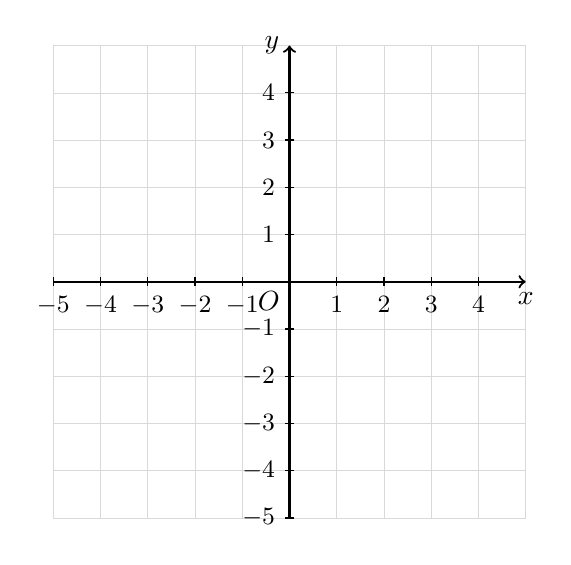
\begin{tikzpicture}[scale=0.6]
    % Grille
    \draw[gray!30, very thin] (-5,-5) grid (5,5);
    
    % Axes
    \draw[thick, ->] (-5,0) -- (5,0) node[anchor=north] {$x$};
    \draw[thick, ->] (0,-5) -- (0,5) node[anchor=east] {$y$};
    
    % Graduation des axes
    \foreach \x in {-5,-4,-3,-2,-1,1,2,3,4}
        \draw (\x,0.1) -- (\x,-0.1) node[below] {\small$\x$};
    \foreach \y in {-5,-4,-3,-2,-1,1,2,3,4}
        \draw (0.1,\y) -- (-0.1,\y) node[left] {\small$\y$};
    
    % Origine
    \draw (0,0) node[below left] {$O$};
    
    % Fonction f(x) = x + 1
   % \draw[Couleur11,very thick, domain=-5:4] plot (\x, {\x + 1});
    
    % Fonction g(x) = 2 (droite horizontale)
  %  \draw[Couleur10,very thick] (-5,2) -- (5,2);
    
    % Fonction h(x) = -3x - 2
    %\draw[Couleur3,very thick, domain=-2.333:1] plot (\x, {-3*\x - 2});
    
    % Fonction k(x) = (3/4)x - 3
   % \draw[Couleur6,very thick, domain=-2.667:5] plot (\x, {0.75*\x - 3});

    
\end{tikzpicture}
\end{center}

\end{minipage}

\end{Exemple}

\section{Sens de variation}

\begin{Propriétés}
Soit $f$ une fonction affine définie par $f(x)=ax+b$, alors :
\begin{itemize}[label=\textcolor{Couleur2}{$\bullet$}]
\item Si $a>0$, $f$ est croissante sur $\R$,
\item Si $a<0$, $f$ est décroissante sur $\R$, 
\item Si $a=0$, $f$ est constante sur $\R$. 
\end{itemize}

\end{Propriétés}

\begin{Remarque}
Soient $m$ et $p$ deux nombres réels tels que $m < p$. $f(p)-f(m) = (ap +b ) - (am + b) = a(p - m)$. \\
On sait que $m < p$ donc $p - m > 0$.
Le signe de $f(p) - f(m)$ est le même que celui de $a$.
\begin{itemize}[label=\textcolor{Couleur7}{$\bullet$}]
\item Si $a>0$, alors $f(p)-f(m)>0$ soit $f(m)<f(p)$.
Donc $f$ est croissante sur $\R$.
\item Si $a<0$, alors $f(p)-f(m)<0$ soit $f(m)>f(p)$.
Donc $f$ est décroissante sur $\R$.
\item Si $a=0$, alors $f(p)-f(m)=0$ soit $f(m)=f(p)$.
\end{itemize}
\end{Remarque}

\begin{Exemples}
\leavevmode\vspace{-\baselineskip}
\begin{itemize}[label=\textcolor{Couleur10}{$\bullet$}]
\item La fonction $f$ définie par $f(x)=3x+2$ est \ligne

\item La fonction $f$ définie par $f(x)=-2x+3$ est \ligne

\item La fonction $f$ définie par $f(x)=5$ est \ligne

\end{itemize}
\end{Exemples}

\newpage

\section{Signe de $f:x\mapsto ax+b$}
\vspace{0.5cm}
Suivant le signe du coefficient directeur $a$, on obtient les tableaux de signes suivants : \\
\begin{minipage}[c]{0.45\linewidth}
\begin{center}
\begin{tikzpicture}[scale=0.9]
\draw (4.5,0.5) node {$a\quad>\quad 0$};
\tkzTabInit[espcl=2,lgt=4]{$x$ / 1 ,variations /1 ,signe de \\$f(x)=ax+b$ /2 } { $-\infty$ , $-\dfrac{b}{a}$ , $+\infty$ };
\tkzTabVar{-/ , R/ , +/};
\tkzTabIma{1}{3}{2}{$0$};
\tkzTabLine{, \color{Couleur8}{-}, z, \color{Couleur3}{+}, };
\end{tikzpicture} 
\end{center}
\end{minipage} \hfill
\begin{minipage}[c]{0.45\linewidth}
\begin{center}
\begin{tikzpicture}[scale=0.9]
\draw (4.5,0.5) node {$a\quad<\quad 0$};
\tkzTabInit[espcl=2,lgt=4]{$x$ / 1 ,variations /1 ,signe de \\$f(x)=ax+b$ /2 } { $-\infty$ , $-\dfrac{b}{a}$ , $+\infty$ };
\tkzTabVar{+/ , R/ , -/};
\tkzTabIma{1}{3}{2}{$0$};
\tkzTabLine{, \color{Couleur3}{+}, z, \color{Couleur8}{-}, };
\end{tikzpicture} 
\end{center}
\end{minipage}
   \vspace{0.5cm}
\begin{center}
\begin{tikzpicture}[scale=1.4]

% Premier graphique : a > 0
\begin{scope}[xshift=0cm]
    % Zones colorées
    \fill[Couleur8!25] (-3,-2) rectangle (3,0);
    \fill[Couleur3!25] (-3,0) rectangle (3,2);
    
    % Axes
    \draw[thick, ->] (-3,0) -- (3,0);
    \draw[thick, ->] (0,-2) -- (0,2);
    
    % Graduations
    \foreach \x in {-2,-1,1,2}
        \draw (\x,0.1) -- (\x,-0.1);
    \foreach \y in {-1,1}
        \draw (0.1,\y) -- (-0.1,\y);
    
    % Origine
    \node[below left] at (0,0) {$0$};
    
    % Droite croissante passant par (-b/a, 0) et (0, b)
    \draw[Couleur6, very thick] (-3,-1) -- (3,2);
    
    % Point d'intersection avec l'axe des x

    \node[below, Couleur6] at (-1,-0.2) {$-\frac{b}{a}$};
    
    % Titre
    \node[above] at (0,2.3) {$a > 0$};
    

\end{scope}

% Deuxième graphique : a < 0
\begin{scope}[xshift=7cm]
    % Zones colorées
    \fill[Couleur3!25] (-3,-2) rectangle (3,0);
    \fill[Couleur8!25] (-3,0) rectangle (3,2);
    
    % Axes
    \draw[thick, ->] (-3,0) -- (3,0);
    \draw[thick, ->] (0,-2) -- (0,2);
    
    % Graduations
    \foreach \x in {-2,-1,1,2}
        \draw (\x,0.1) -- (\x,-0.1);
    \foreach \y in {-1,1}
        \draw (0.1,\y) -- (-0.1,\y);
    
    % Origine
    \node[below left] at (0,0) {$0$};
    
    % Droite croissante passant par (-b/a, 0) et (0, b)
    \draw[Couleur6, very thick] (-3,1) -- (3,-2);
    
    % Point d'intersection avec l'axe des x
    \node[below, Couleur6] at (-1,-0.2) {$-\frac{b}{a}$};
    
    % Titre
    \node[above] at (0,2.3) {$a < 0$};
    

\end{scope}

\end{tikzpicture}
\end{center}

\vspace{0.5cm}
\begin{Exemple}
Tableau de signes des fonctions définies sur $\R$ par $f(x)=2x+4$ et $g(x)=-x+3$ :\\

\vspace{6cm}

\end{Exemple}   

\newpage
\section{Méthodes}

\subsection{Déterminer les coefficients à partir de la représentation graphique}

\begin{Propriété}
Si $A(x_A ; y_A)$ et $ B(x_B ; y_B)$ sont deux points distincts de la droite $(d)$ représentant la
fonction $f$ définie sur $\R$ par $f(x)=ax+b$ alors : $a=\dfrac{y_B-y_A}{x_B-x_A}$
\end{Propriété}




\begin{Méthodes}
\leavevmode\vspace{-\baselineskip}
\begin{center}
\begin{tikzpicture}[scale=0.6]
    % Grille
    \draw[gray!30, very thin] (-5,-5) grid (5,5);
    
    % Axes
    \draw[thick, ->] (-5,0) -- (5,0) node[anchor=north] {$x$};
    \draw[thick, ->] (0,-5) -- (0,5) node[anchor=east] {$y$};
    
    % Graduation des axes
    \foreach \x in {-5,-4,-3,-2,-1,1,2,3,4}
        \draw (\x,0.1) -- (\x,-0.1) node[below] {\small$\x$};
    \foreach \y in {-5,-4,-3,-2,-1,1,2,3,4}
        \draw (0.1,\y) -- (-0.1,\y) node[left] {\small$\y$};
    
    % Origine
    \draw (0,0) node[below left] {$O$};
    
    % Fonction f(x) = 2x + 2
    \draw[Couleur8,very thick, domain=-3.5:1.5] plot (\x, {2*\x + 2});
\draw (2,4.5) node {\color{Couleur8}{$(d')$}};
    
    % Fonction g(x) = -0.5x - 1
    \draw[Couleur6,very thick, domain=-5:5] plot (\x, {-0.5*\x - 1});
  \draw (4.5,-2.5) node {\color{Couleur6}{$(d)$}};
    
    % Points
   % \fill[violet] (0,2) circle (3pt) ;
    % \fill[Couleur10] (0,-1) circle (3pt);
    
% \draw[Couleur3, thick, ->] (-3,-4) -- (-2,-4) node[midway, below] {\color{Couleur3}{+1}};
    
       % \draw[Couleur3, thick, ->] (-2,-4) -- (-2,-2) node[midway, right] {\color{Couleur3}{+2}};
        
      %  \draw[Couleur11, thick, ->] (2,-3) -- (4,-3) node[midway, below] {\color{Couleur11}{+2}};
    
      %  \draw[Couleur11, thick, ->] (2,-2) -- (2,-3) node[midway, left] {\color{Couleur11}{-1}};
    
\end{tikzpicture}
\end{center}
\begin{itemize}[label=\textcolor{Couleur3}{$\bullet$}]
\begin{multicols}{2}
\item Pour $(d')$ : \\
Le coefficient directeur est \ligne

L'ordonnée à l'origine est \ligne

La fonction $f$ représentée par la droite $(d')$ est \\
définie par \ligne

\item Pour $(d)$ : \\
Le coefficient directeur est \ligne

L'ordonnée à l'origine est \ligne

La fonction $g$ représentée par la droite $(d)$ est \\
définie par \ligne

\end{multicols}
\end{itemize}
\vspace{-0.8cm}
\end{Méthodes}

\vspace{0.3cm}
\subsection{Déterminer l'expression d'une fonction affine}

\begin{Méthodes}Déterminer une fonction affine par le calcul \\
Déterminer par le calcul une expression de la fonction $f$ telle que $f (-2) = 4$ et $f (3) = 1$.
\vspace{0.1cm}

\ligne

\ligne

\ligne

\ligne

\ligne

\ligne

\ligne

\ligne

\ligne

\ligne

\ligne

\begin{Remarque}
Le graphique permet de lire des valeurs approchées de $a$ et $b$.
Cette méthode graphique n'est pas précise mais permet d'avoir un ordre de grandeur des valeurs cherchées.
\end{Remarque}
\end{Méthodes}

\bigskip

\newpage

\section*{Exercices - Fonctions affines}
\addcontentsline{toc}{section}{Exercices}
{\setlength{\columnseprule}{0pt}
\setcounter{NumEx}{1}

\subsection*{Généralités}


\begin{Exercice} %1
Déterminer, en expliquant, si les fonctions suivantes sont, ou non, des fonctions affines. Si oui, donner leur coefficient directeur et leur ordonnée à l'origine.
\vspace{-0.5cm}
\begin{multicols}{3}
\begin{enumerate}

\item $f(x)=9x^{2}+13 $.
\item $f(x)=2 +6  x$.
\item $f(x)=6x+1$
\item $f(x)=\sqrt{7}x + \sqrt{10}$.
\item $f(x)=10\times (-2x-8) $.
\item $f(x)=\dfrac{-2x+4}{3}$.
\end{enumerate}
\end{multicols}
\end{Exercice}



\begin{Exercice} %2
\begin{minipage}[c]{0.5\linewidth}
   Pour chacune des fonctions affines suivantes, déterminer a et b puis représenter les graphiquement :
      \begin{itemize}[label=\textcolor{Couleur6}{$\bullet$}]
       \item $f(x)=-2x+1$ , $ a=...\text{ et } b=... $
         \item $g(x)=\dfrac{2}{3}x-1$ $ a=...\text{ et } b=... $
         \item $h(x)=2$ $ a=...\text{ et } b=... $
         \item $k(x)=3x+3$ $ a=...\text{ et } b=... $
      \end{itemize}
\end{minipage} \hfill
\begin{minipage}[c]{0.5\linewidth}
\begin{center}
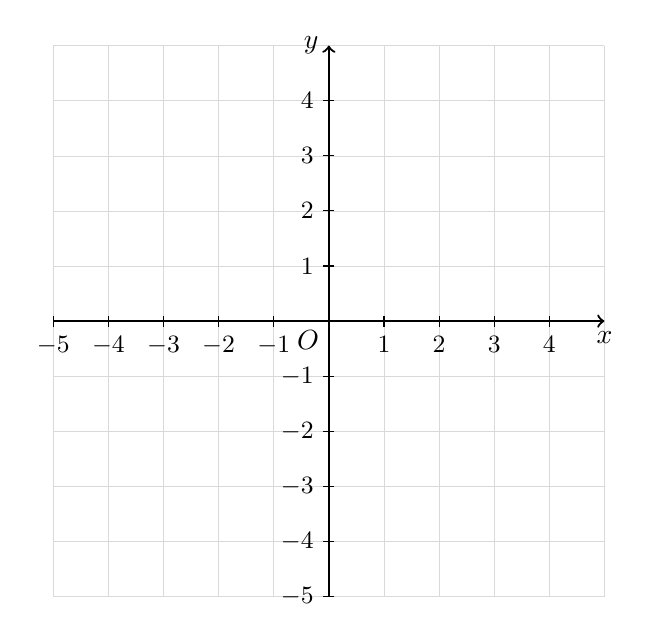
\begin{tikzpicture}[scale=0.7]
    % Grille
    \draw[gray!30, very thin] (-5,-5) grid (5,5);
    
    % Axes
    \draw[thick, ->] (-5,0) -- (5,0) node[anchor=north] {$x$};
    \draw[thick, ->] (0,-5) -- (0,5) node[anchor=east] {$y$};
    
    % Graduation des axes
    \foreach \x in {-5,-4,-3,-2,-1,1,2,3,4}
        \draw (\x,0.1) -- (\x,-0.1) node[below] {\small$\x$};
    \foreach \y in {-5,-4,-3,-2,-1,1,2,3,4}
        \draw (0.1,\y) -- (-0.1,\y) node[left] {\small$\y$};
    
    % Origine
    \draw (0,0) node[below left] {$O$};
    
\end{tikzpicture}
\end{center}
\end{minipage}
\\

\end{Exercice}

\subsection*{Variations}


\begin{Exercice} %3
Déterminer le sens de variation de la fonction :
\vspace{-0.5cm}
\begin{multicols}{2}
\begin{enumerate}
	\item $f$ définie sur $[-3\,;\,8]$ par : $f(x)=3x$.
	\item $v$ définie sur $\mathbb R$ par : $v(x)=5x+2$.
	\item $u$ définie sur $[-5\,;\,3]$ par : $u(x)=8-8x$.
	\item $g$ définie sur $\mathbb R$ par : $g(x)=\dfrac{3-6x}{4}$.
	\item $h$ définie sur $\mathbb R$ par : $h(x)=\dfrac{-2+5x}{6}$.
	\item $w$ définie sur $\mathbb R$ par : $w(x)=-9x+1$.
	\item $w$ définie sur $\mathbb R$ par : $w(x)=-5x-7$.
	\item $f$ définie sur $[1\,;\,7]$ par : $f(x)=-4x$.
	\item $f$ définie sur $\mathbb R$ par : $f(x)=\dfrac{-x-8}{9}$.
	\item $u$ définie sur $\mathbb R$ par : $u(x)=-2+7x$.
\end{enumerate}
\end{multicols}
\end{Exercice}

\newpage

\subsection*{Signe}


\begin{Exercice} %4
Déterminer le tableau de signe des fonctions de l'exercice 3.
\end{Exercice}



\begin{Exercice} %5
\leavevmode\vspace{-\baselineskip}
\begin{enumerate}[itemsep=1.75em]
	\item \begin{minipage}[t]{\linewidth}Une fonction affine $u$  définie sur $\mathbb R$ est strictement croissante. De plus $u(-8)=0$.\\
        \textbf {a.}  Dresser son tableau de signes sur $\mathbb R$.\\
        \textbf {b.}  Donner une fonction $u$ vérifiant les conditions précédentes.\end{minipage}
	\item \begin{minipage}[t]{\linewidth}Une fonction affine $w$  définie sur $\mathbb R$ est strictement décroissante. De plus $w(-0{,}4)=0$.\\
        \textbf {a.}  Dresser son tableau de signes sur $\mathbb R$.\\
        \textbf {b.}  Donner une fonction $w$ vérifiant les conditions précédentes.\end{minipage}
	\item \begin{minipage}[t]{\linewidth}Une fonction affine $u$  définie sur $\mathbb R$ vérifie $u(2)=0$ et $u(-1)=9$.\\
           Dresser son tableau de signes sur $\mathbb R$. Justifier.
         \end{minipage}
	\item \begin{minipage}[t]{\linewidth}Une fonction affine $h$  définie sur $\mathbb R$ vérifie $h(-1)=0$ et $h(-2)=-1$.\\
           Dresser son tableau de signes sur $\mathbb R$. Justifier.
         \end{minipage}
\end{enumerate}
\end{Exercice}

\begin{Exercice} %6
\leavevmode\vspace{-\baselineskip}
\begin{enumerate}[itemsep=1.75em]
	\item \begin{minipage}[t]{\linewidth}On donne le tableau de signes d'une fonction affine  $f$  définie sur $\mathbb R$ :\\\begin{tikzpicture}[baseline, scale=0.75]
    \tkzTabInit[lgt=5,deltacl=0.8,espcl=5]{ $x$ / 1.5, $f(x)$ / 2}{ $-\infty$, $6$, $+\infty$}
	\tkzTabLine{  , +, z, -}
	\end{tikzpicture}
\\ \textbf {a.}  Donner le sens de variation de $f$ sur $\mathbb R$.\\
        \textbf {b.}  Comparer $f(10)$ et $f(8)$.\end{minipage}
        \newpage
	\item \begin{minipage}[t]{\linewidth}On donne le tableau de signes d'une fonction affine  $f$  définie sur $\mathbb R$ :\\\begin{tikzpicture}[baseline, scale=0.75]
    \tkzTabInit[lgt=5,deltacl=0.8,espcl=5]{ $x$ / 1.5, $f(x)$ / 2}{ $-\infty$, $5$, $+\infty$}
	\tkzTabLine{  , -, z, +}
	\end{tikzpicture}
\\ \textbf {a.}  Donner le sens de variation de $f$ sur $\mathbb R$.\\
        \textbf {b.}  Comparer $f(2)$ et $f(4)$.\end{minipage}
\end{enumerate}
\end{Exercice}

\newpage

\subsection*{Méthodes}

\begin{Exercice} %7
   Pour chacune des fonctions affines suivantes, déterminer graphiquement son expression :\\
   
\begin{minipage}[c]{0.4\linewidth}
\begin{center}
\begin{tikzpicture}[scale=0.7]
% Définition des limites
\def\xmin{-5}
\def\xmax{5}
\def\ymin{-5}
\def\ymax{5}

% Axes
\draw[->] (\xmin,0) -- (\xmax,0) node[right] {$x$};
\draw[->] (0,\ymin) -- (0,\ymax) node[above] {$y$};

% Repères
\draw (0,0) node[below left] {0};
\draw (1,0) node[below] {1};
\draw (0,1) node[left] {1};

% Grille
\draw[dotted, gray] (\xmin,\ymin) grid (\xmax,\ymax);

% Courbes avec domaines calculés pour rester dans le repère
\draw[samples=300,domain=-0.33:3,violet,thick] plot(\x,-3*\x+4);
\draw[samples=300,domain=-5:5,Couleur8,thick] plot(\x,-2);
\draw[samples=300,domain=-1.5:1,Couleur3,thick] plot(\x,4*\x+1);
\draw[samples=300,domain=-2.5:5,Couleur6,thick] plot(\x,4/5*\x-3);

% Étiquettes
\draw [color=Couleur8](1.5,-1.5) node {$\mathcal{C}_f$};
\draw [color=violet](0.5,2.5) node {$\mathcal{C}_g$};
\draw [color=Couleur3](-2,2) node {$\mathcal{C}_h$};
\draw [color=Couleur6](3,0) node {$\mathcal{C}_k$};
\end{tikzpicture}
\end{center}
\end{minipage}
\hfill
\begin{minipage}[c]{0.4\linewidth}
\begin{center}
\begin{tikzpicture}[scale=0.7]
% Définition des limites
\def\xmin{-5}
\def\xmax{5}
\def\ymin{-5}
\def\ymax{5}

% Axes
\draw[->] (\xmin,0) -- (\xmax,0) node[right] {$x$};
\draw[->] (0,\ymin) -- (0,\ymax) node[above] {$y$};

% Repères
\draw (0,0) node[below left] {0};
\draw (1,0) node[below] {1};
\draw (0,1) node[left] {1};

% Grille
\draw[dotted, gray] (\xmin,\ymin) grid (\xmax,\ymax);

% Courbes avec domaines calculés pour rester dans le repère
\draw[samples=300,domain=-3:2,pink,thick] plot(\x,2*\x+1);
\draw[samples=300,domain=-5:5,Couleur8,thick] plot(\x,-1);
\draw[samples=300,domain=-2:5,Couleur3,thick] plot(\x,-1*\x+3);
\draw[samples=300,domain=-2.67:4,Couleur6,thick] plot(\x,3/2*\x-1);

% Étiquettes
\draw [color=Couleur8](1.5,-0.5) node {$\mathcal{C}_{f_1}$};
\draw [color=pink](0.5,2.5) node {$\mathcal{C}_{g_1}$};
\draw [color=Couleur3](-2,2) node {$\mathcal{C}_{h_1}$};
\draw [color=Couleur6](3,1) node {$\mathcal{C}_{k_1}$};
\end{tikzpicture}
\end{center}
\end{minipage}



\end{Exercice}





\begin{Exercice} %8
Une fonction $ f $, définie sur $ \R $ et telle que $f(0)=3$, $f(2)=5$ et $f(3)=7$ peut-elle être affine ?
\end{Exercice}

\begin{Exercice} %9
Vrai ou faux ? Une fonction $g$ telle que $g(-1) = -2$, $g(2) = 10$ et $g(21) = 88$ est forcément affine.
\end{Exercice}

\begin{Exercice} %10
(Challenge) Soit $a$ et $b$ deux réels et $f$ une fonction définie sur $\R$ par $f (x) = ax + b$. On sait que la droite qui représente cette fonction coupe l'axe des abscisses au point d'abscisse 2 et l'axe des ordonnées en un point dont l'ordonnée se trouve dans
l'intervalle $] - 2; 1[$. Quelles sont les valeurs possibles de $a$ et $b$ ?
\end{Exercice}


\begin{Exercice} %11
Dans chaque cas, déterminer l'expression algébrique de la fonction affine $f$ définie sur $\mathbb R$ ...
\begin{enumerate}[itemsep=0.5em]
	\item Sachant que $f(5)=14$ et que $f(2)=11$. 
	\item Sachant que $f(9)=-27$ et que $f(4)=-8$.
	\item Passant par les points $A(9;-26)$ et $B(2;-18)$.
	\item Sachant que $f(6)=5$ et que $f(2)=-5$.
	\item Passant par les points $A(1;-4)$ et $B(3;-10)$.
	\item Sachant que $f(9)=-19$ et que $f(2)=-5$.
	\item Sachant que $f(5)=20$ et que $f(4)=17$.
	\item Passant par les points $A(4;0)$ et $B(3;-26)$.
\end{enumerate}
\end{Exercice}

\newpage

\subsection*{Bilan}

\begin{Exercice} %12
Deux cyclistes font une course sur une distance de 100 km. Le premier effectue le parcours à une vitesse de 40 km/h. Le second fait la première moitié de la course à 50 km/h et la deuxième à une vitesse de 30 km/h. Au temps $t$, on appelle $d_1(t)$ et $d_2(t)$ les distances parcourues par ces deux cyclistes.
\begin{enumerate}
\item Représenter la courbe de la fonction $d_1$ dans un repère orthogonal (on prendra un carreau = 10 km en ordonnée et 6 carreaux = 1 heures en abscisse).
\item Sur ce même repère, représente la courbe de la fonction $d_2$
\item A quel instant les deux cyclistes se croisent-ils ?
\item Qui semble arriver en premier ?
\item (Challenge) Retrouver algébriquement les résultats à ces questions.
\end{enumerate}
\end{Exercice}


\begin{Exercice} %13
Un médecin généraliste évalue ainsi son chiffre d'affaire et ses dépenses :
\begin{itemize}[label=\textcolor{Couleur6}{$\bullet$}]
\item Ses charges fixes sont de 18 000 € par an.
\item Une consultation au tarif classique est payée 25 €, mais le médecin en reverse environ 9 \% pour le compte de l'URSSAF et 23\% pour la CARMF. Ce médecin souhaite alors organiser au mieux son année.
\end{itemize}

\begin{enumerate}
\item Soit $n$ le nombre de consultation du médecin à l'année. Exprimer $C(n)$, le chiffre d'affaire du médecin, en fonction de $n$.
\item Combien de consultations doit-il réaliser pour gagner au moins 36 000 € annuels ?
\item S'il travaille 47 semaines par an, 4 jours par semaine, combien de consultations
journalières cela représente-t-il ?
\end{enumerate}
\end{Exercice}


}
